\documentclass[compress]{beamer}
\mode<presentation>

\usetheme{Warsaw}
\definecolor{innotek}{RGB}{2,52,173}
\setbeamercolor*{palette primary}{use=structure,fg=white,bg=innotek}
%\usecolortheme[RGB={2,52,173}]{structure}
\defbeamertemplate*{footline}{shadow theme}
{%
  \leavevmode%
  \hbox{\begin{beamercolorbox}[wd=.5\paperwidth,ht=2.5ex,dp=1.125ex,leftskip=.3cm plus1fil,rightskip=.3cm]{author in head/foot}%
    \usebeamerfont{author in head/foot}\hfill\insertshortauthor%
  \end{beamercolorbox}%
  \begin{beamercolorbox}[wd=.5\paperwidth,ht=2.5ex,dp=1.125ex,leftskip=.3cm,rightskip=.3cm plus1fil]{title in head/foot}%
      \usebeamerfont{title in head/foot}\insertshorttitle\hfill\insertframenumber\,/\,\inserttotalframenumber%
  \end{beamercolorbox}}%
  \vskip0pt%
}
\setbeamertemplate{navigation symbols}{}%remove navigation symbols

\usepackage{subfigure}
\usepackage{multicol}
%\usepackage{amsmath}
\usepackage{epsfig}
\usepackage{graphicx}
\usepackage[all,knot]{xy}
\xyoption{arc}
\usepackage{url}
\usepackage{multimedia}
\usepackage{hyperref}
\usepackage{setspace}

% define your own colours:
\definecolor{innotek}{RGB}{1,54,160}
\definecolor{Red}{rgb}{1,0,0}
\definecolor{Blue}{rgb}{0,0,1}
\definecolor{Green}{rgb}{0,1,0}
\definecolor{magenta}{rgb}{1,0,.6}
\definecolor{lightblue}{rgb}{0,.5,1}
\definecolor{lightpurple}{rgb}{.6,.4,1}
\definecolor{gold}{rgb}{.6,.5,0}
\definecolor{orange}{rgb}{1,0.4,0}
\definecolor{hotpink}{rgb}{1,0,0.5}
\definecolor{newcolor2}{rgb}{.5,.3,.5}
\definecolor{newcolor}{rgb}{0,.3,1}
\definecolor{newcolor3}{rgb}{1,0,.35}
\definecolor{darkgreen1}{rgb}{0, .35, 0}
\definecolor{darkgreen}{rgb}{0, .6, 0}
\definecolor{darkred}{rgb}{.75,0,0}

\xdefinecolor{olive}{cmyk}{0.64,0,0.95,0.4}
\xdefinecolor{purpleish}{cmyk}{0.75,0.75,0,0}

\useoutertheme[subsection=false]{smoothbars}

\title{POW-R}
\subtitle{Power Outlet Wireless Reporter}
\author[]{Grace De Geus\\Charles Hathaway\\Forest Immel\\Nate Pickett\\Niloc Quimby}
\date{December $7^{th}$, 2012}

\begin{document}

\frame{
    \titlepage
}


\section{Architecture}
\subsection{XBee Radios}

\frame{
 \frametitle{Why XBee Radios?}
  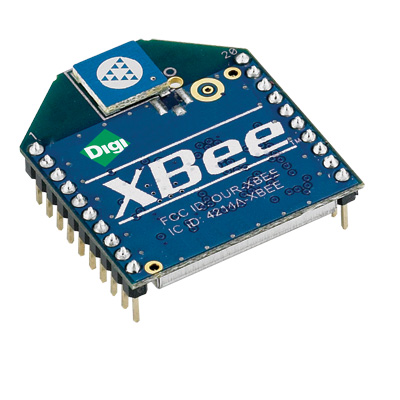
\includegraphics[scale=.16 ]{images/xBee.jpg}
 \begin{itemize}
  \item Small form factor (just larger than U.S. quarter)
  \item Low power consumption (\textasciitilde .1 W)
  \item Talk over ZigBee protocol
 \end{itemize}
}

\frame{
 \frametitle{ZigBee}
 \begin{itemize}
  \item Prototyping hardware
  \item ZigBee specification  
 \end{itemize}
}
\subsection{Server and Coordinator}

\frame{
 \frametitle{Coordinator Design}
  Must:
 \begin{itemize}
		\item Host Coordinator XBee
		\item Host LCD to display IP
		\item Listen for readings
		\item Send readings to Server
 \end{itemize}
}

\frame{
 \frametitle{Coordinator Implementation}
 Arduino:
 \begin{itemize}
	\item Talks to LCD using SoftwareSerial
	\item Listens for readings from XBee
	\item Sends readings over USB cable
 \end{itemize}
}

\frame{
 \frametitle{Server Design}
 Server must:
 \begin{itemize}
  \item Be small
  \item Consume as little power as possible
  \item Listen for readings from Coordinator 
  \item Store readings
  \item Host all of the Display
 \end{itemize}
}

\frame{
 \frametitle{Server Implementation}
  Raspberry Pi:
 \begin{itemize}
  \item Small form factor (\textasciitilde 8.5 x 5.6 cm)
  \item Low power consumption (\textasciitilde 3.5 W)
  \item Acts as data center and web server for Display
 \end{itemize}
}



\section{Closing}
\subsection{Reflection}

\frame{
 \frametitle{Lessons Learned}
	\begin{itemize}
		\item Order parts ASAP
		\item Understanding new material
		\item Team dynamics
		\item Time management
	\end{itemize}
 }

\frame{
 \frametitle{How would we do it all over again?}
    \begin{itemize}
		\item Start development sooner
		\item Stick to schedule
	\end{itemize}
}

\frame{
 \frametitle{Future plans, potential improvements}
    \begin{itemize}
		\item Satellite functionality
		\item Home Automation Framework
	\end{itemize}
}
\subsection{Demonstration}

\frame{
 \frametitle{Demonstration time!}
	\begin{center}
	{\huge Check it out!}
	\end{center}
 }

\frame{
 \frametitle{Questions and Closing}
    \begin{center}
        {\huge Questions?}
        
        {\small Presentation made using \LaTeX{} }

		
		Our website: \url{http://powr.logrit.com/}
		
    \end{center}
}

\end{document}

